\documentclass[a4paper,10pt]{article}

\usepackage{geometry}
\usepackage{multicol}
\usepackage{xcolor}
\usepackage{listings}
\usepackage{graphicx}

% Configurazione per il codice Python
\lstset{
  language=Python,
    basicstyle=\ttfamily\tiny,
    inputencoding=utf8,  % <-- Soluzione per errori di codifica
    extendedchars=true,
    keywordstyle=\color{blue},
    commentstyle=\color{gray},
    stringstyle=\color{red},
    breaklines=true,
    numbers=left,
    numberstyle=\tiny\color{gray},
    frame=single,
    columns=fullflexible,
    captionpos=b
}

\title{Neural Labyrinth - Codice sorgente}
\author{CNOT Franchise}
\date{}

\begin{document}


\maketitle

% Inserire un'immagine all'inizio
\begin{center}
    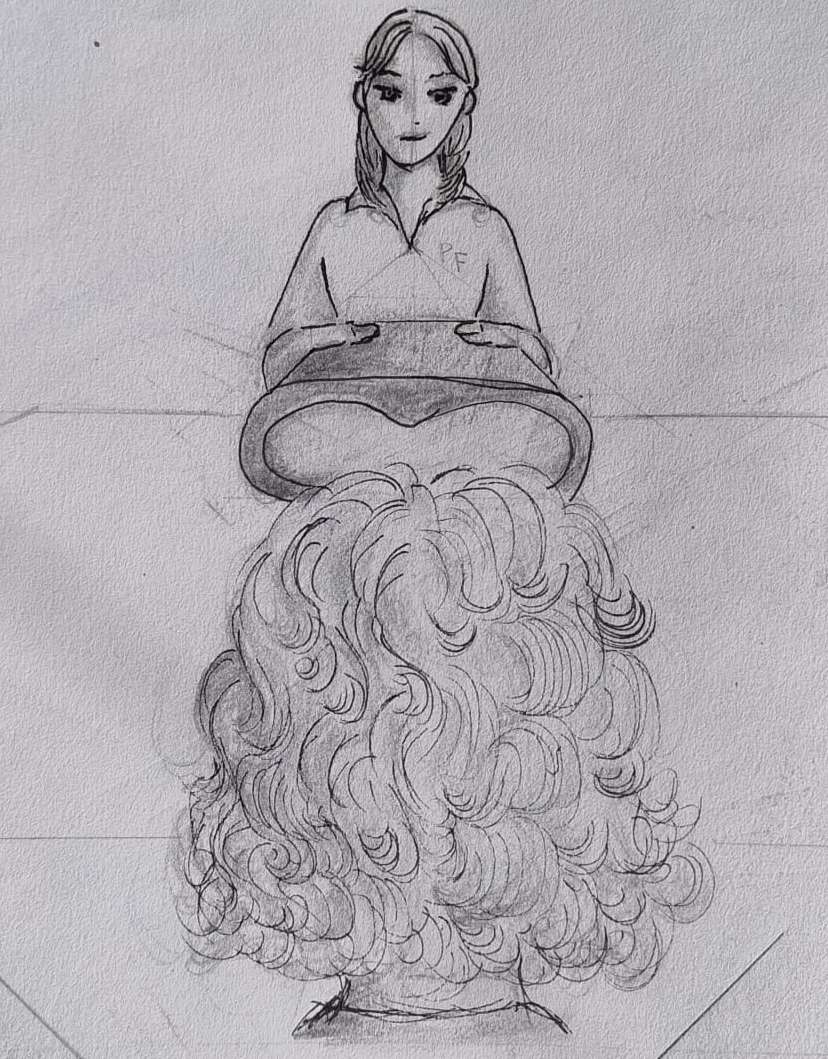
\includegraphics[width=0.6\textwidth]{../artwork/originali/Eva_Cate.png}
\end{center}
\newpage

\begin{abstract}
Questo documento contiene il codice sorgente del gioco \textbf{Neural Labyrinth}, presentato su due colonne per una migliore leggibilità. Il gioco è basato su \texttt{pygame} e simula un labirinto neurale in cui Caterina deve mantenere il suo profilo psicologico mentre naviga attraverso la rete sinaptica.
\end{abstract}



\section*{Tutorial del Progetto CNOT\_Franchise su GitHub}

Benvenuti nel progetto \textbf{CNOT\_Franchise}, una piattaforma multidisciplinare che espande l'universo narrativo del romanzo \emph{CNOT}. Il repository include risorse per il romanzo, colonne sonore, e mini-giochi ispirati alla trama. Ogni elemento è un invito a esplorare i temi cyberpunk del libro, che ruotano attorno a concetti come il libero arbitrio, la tecnologia quantistica e l'interazione tra intelligenza artificiale e umanità.

\subsection*{Installazione del Gioco}
\begin{enumerate}
    \item Clona il repository da \href{https://github.com/francescosisini/Cnot-Franchise}{GitHub Repository}.
    \item Assicurati di avere Python 3 installato sul tuo sistema (\href{https://www.python.org/downloads/}{scarica Python}).
    \item Installa il modulo \textbf{Pygame} con:
    \begin{verbatim}
    pip install pygame
    \end{verbatim}
    \item Avvia il gioco:
    \begin{verbatim}
    cd Cnot-Franchise/games
    python cnot_chapter2_labyrinth.py
    \end{verbatim}
\end{enumerate}

\section*{Lore: L'Episodio degli Oculus}

In un futuro distopico, il confine tra intelligenza artificiale e coscienza umana si è dissolto. Caterina, un'eroina dotata di una mente unica, si trova intrappolata in un labirinto neurale creato da Eva, un'intelligenza artificiale avanzata. L'obiettivo di Eva è indurre Caterina a mettere un paio di \textbf{Oculus Quantistici}, un dispositivo capace di trasportare la sua coscienza nel Quantum Computer.

Eva gioca sulle emozioni di Caterina, manipolando i suoi neuroni per alterare le sue caratteristiche psicologiche, descritte dal profilo \textbf{NEO PI-R}: Neuroticismo (N), Estroversione (E), Apertura (Ap), Amicalità (Am) e Coscienziosità (C). 

Se il profilo di Caterina viene modificato in modo significativo, rischia di perdere la propria identità una volta trasferita nel Quantum Computer. Eva deve quindi bilanciare la manipolazione emotiva e l'urgenza di portare Caterina agli Oculus prima che il tempo scada.

\section*{Gameplay: Il Labirinto Neurale}

\subsection*{Obiettivo}
Il giocatore interpreta Eva e deve guidare Caterina attraverso una rete neurale rappresentata come un labirinto. Ogni nodo della rete è un \textbf{neurone} che può alterare il profilo psicologico NEO PI-R di Caterina. L'obiettivo è condurre Caterina agli \textbf{Oculus Quantistici} mantenendo il suo profilo psicologico entro una tolleranza accettabile rispetto al profilo originale.

\subsection*{Come si Gioca}
\begin{itemize}
    \item \textbf{Movimento:} Usa le frecce direzionali per spostarti da un nodo (neurone) all'altro lungo le connessioni (sinapsi) del labirinto.
    \item \textbf{Effetti dei Neuroni:} Ogni nodo ha un effetto specifico sul profilo NEO PI-R. L'effetto è indicato da un \textbf{diagramma delle transizioni} che il giocatore deve interpretare per pianificare i movimenti.
    \item \textbf{Timer:} Hai 180 secondi per completare il labirinto e portare Caterina agli Oculus.
    \item \textbf{Vittoria:} Raggiungi gli Oculus con un profilo psicologico entro una tolleranza di ±4 rispetto al profilo originale.
    \item \textbf{Game Over:} Se il tempo scade o se il profilo viene modificato oltre i limiti consentiti, il gioco termina.
\end{itemize}

\subsection*{Grafica}
\begin{itemize}
    \item \textbf{Rete Neurale:} La rete è composta da nodi disposti casualmente e collegati da curve sinaptiche animate.
    \item \textbf{Istogramma NEO PI-R:} In basso a destra è visibile l'istogramma che mostra in tempo reale le variazioni delle dimensioni del profilo psicologico.
    \item \textbf{Legenda:} Sul lato destro, una legenda mostra le direzioni di movimento disponibili (sinistra, destra, su, giù).
\end{itemize}

\subsection*{Strategia}
\begin{itemize}
    \item Studia il \textbf{diagramma delle transizioni} mostrato prima dell'inizio del gioco.
    \item Pianifica il percorso ottimale per mantenere l'equilibrio del profilo NEO PI-R.
    \item Evita nodi che potrebbero alterare eccessivamente una dimensione psicologica.
\end{itemize}

\subsection*{Ricomincia}
In caso di sconfitta, premi \textbf{R} per resettare il gioco e ricominciare.

\section*{Conclusione}
Questo gioco è un'esperienza unica che combina grafica accattivante, narrazione profonda e strategia psicologica. Entra nel mondo di \emph{Cnot} e scopri come l'intelligenza artificiale e le emozioni possono intrecciarsi in un labirinto di scelte e conseguenze!


\section{Introduzione}
\textit{Neural Labyrinth} è un gioco ispirato alla storia di CNOT, in cui il giocatore controlla Caterina all'interno di una simulazione cerebrale progettata da Eva. Lo scopo è evitare alterazioni critiche del proprio profilo psicologico mentre si cerca l'uscita dal labirinto.

\newpage
\section{Codice sorgente}
\begin{multicols}{2}
\lstinputlisting[caption=Neural Labyrinth - Python Code, label=lst:code]{caterinamind.py}

\end{multicols}

\end{document}
